\documentclass[a4paper,11pt]{report}
\usepackage[T1]{fontenc}
\usepackage[utf8]{inputenc}
\usepackage{lmodern}
\usepackage[francais]{babel}
\usepackage{graphicx}
\usepackage{array}

\title{Data wars }

\author{Guillaume LAROYENNE, Nathan PRETOT \\ Jeremy RENAUD, Tom SALVI, Pierre VALENZA}

\begin{document}

\maketitle
\tableofcontents

\chapter{Guide du joueur}

	\section{Inscription}
        Depuis le site vous trouverez en haut à droite de votre écran un bouton rouge "S'inscrire", cliquer et remplisser les champs correctement. 

	\section{Connexion}
        Depuis le site vous trouverez en haut à droite de votre écran un bouton bleu "Se connecter", cliquer et remplisser les champs correctement. 

	\section{Modifier mon deck}
       	Une fois connecter vous êtes rediriger sur la gestion de votre deck, sinon cliquer sur le bouton mon deck dans la barre de navigation. 

	\begin{figure}[th]
		\begin{center}
		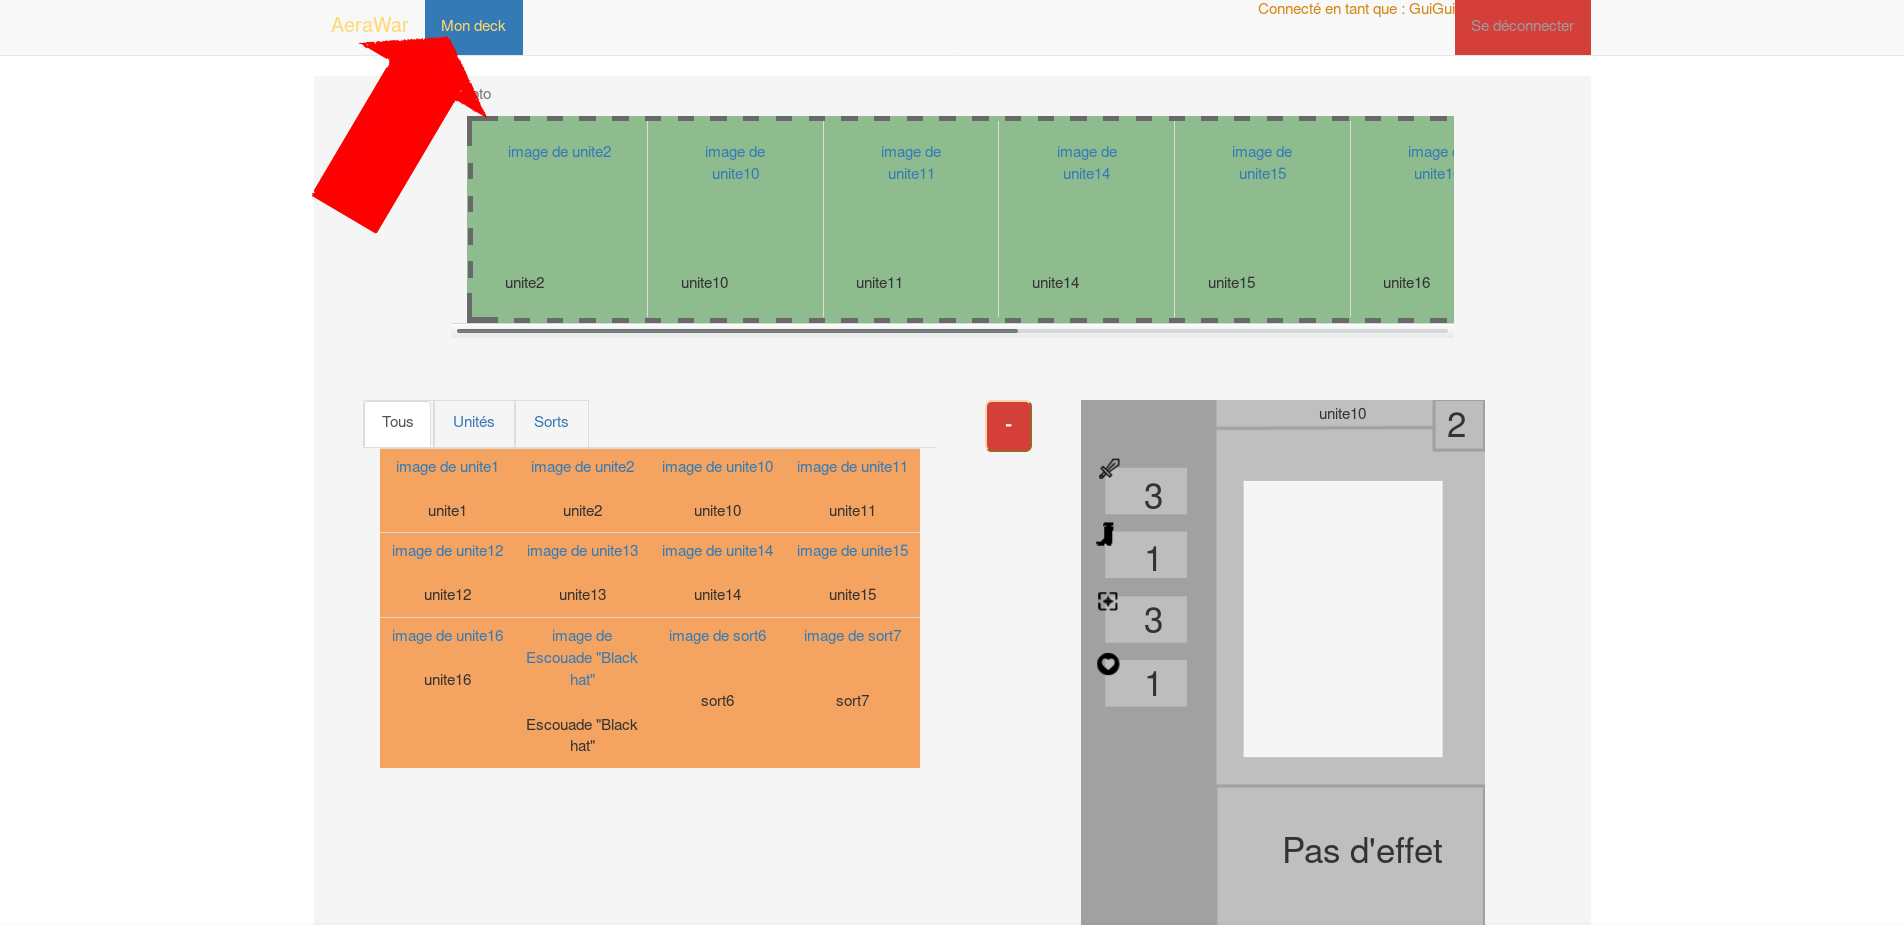
\includegraphics[scale=0.4]{Assets/go_deck.png}
      		\caption{Afficher son deck \textit{data wars}}
      		\label{fig1}
     		\end{center}
	\end{figure}

	Maintenant selectionner une carte, peut importe si elle est présente dans votre deck. 	Vous allez remarquer que la carte c'est afficher sur la partie droite de l'écran.

	\begin{figure}[th]
		\begin{center}
		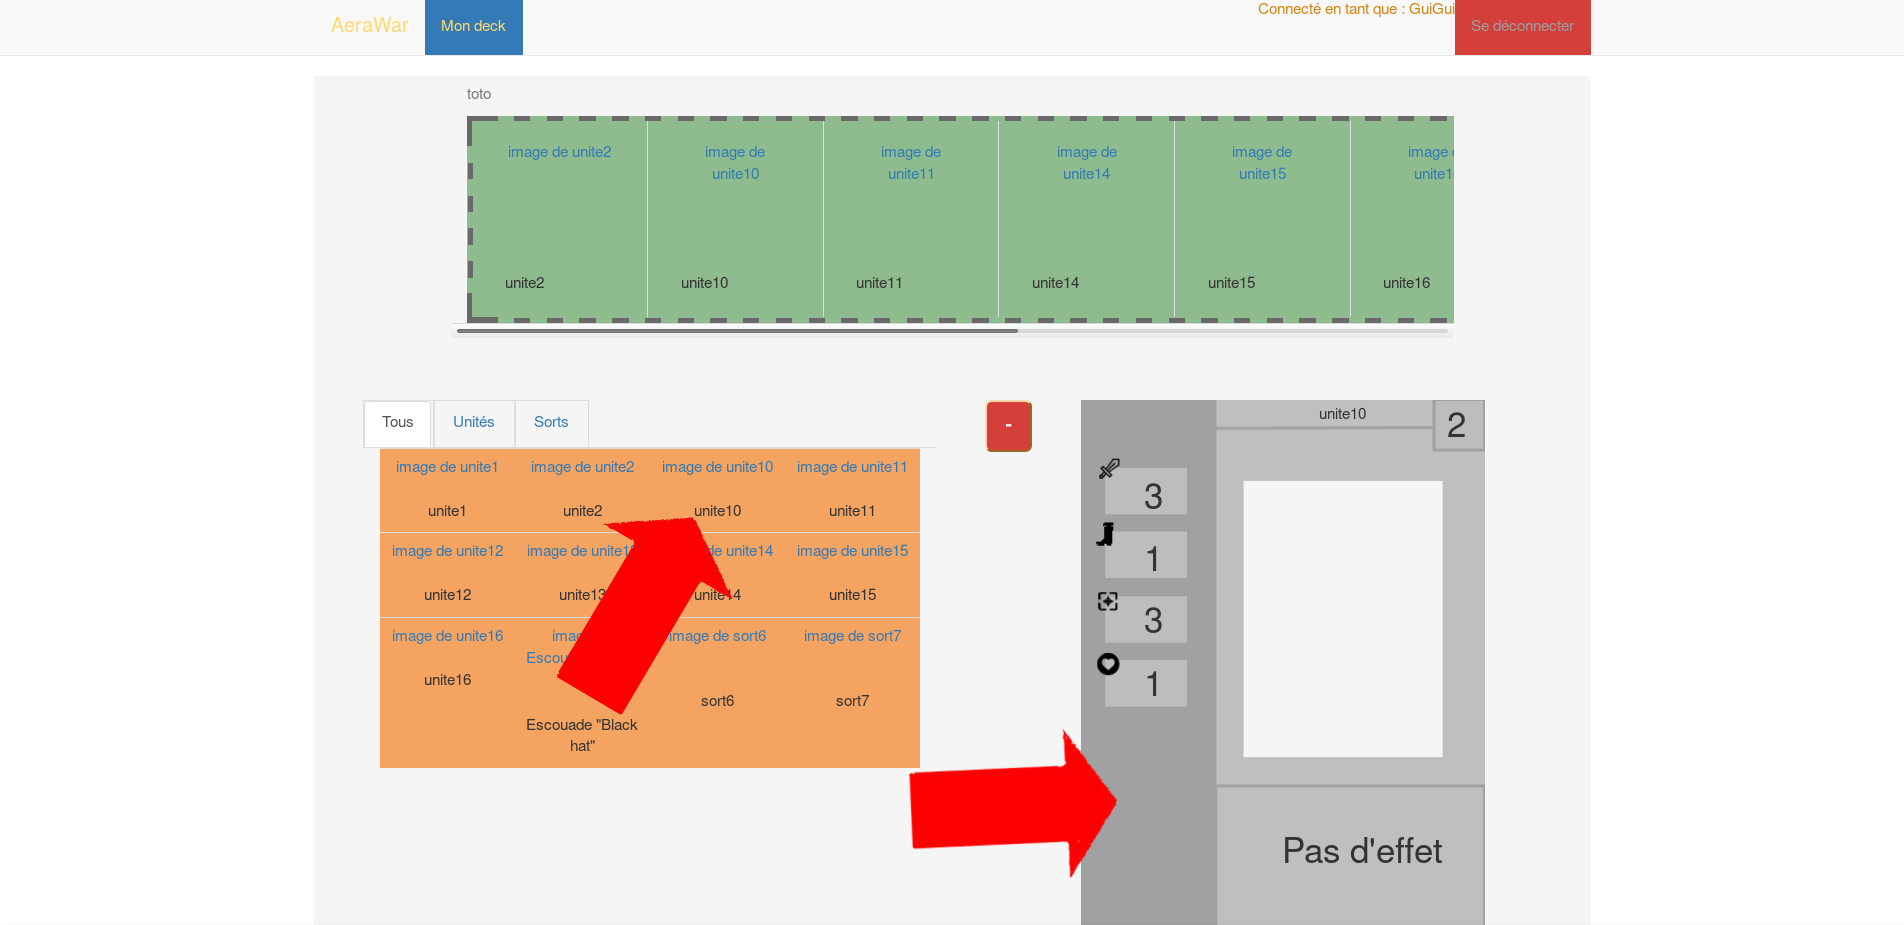
\includegraphics[scale=0.4]{Assets/carte_deck.png}
      		\caption{Selection d'une carte \textit{data wars}}
      		\label{fig2}
     		\end{center}
	\end{figure}

	A partir d'ici vous pouvez ajouter ou enlever la carte de votre deck.
RAPPEL : vous ne pouvez avoir plus de 15 cartes dans votre deck et une carte ne peut apparaitre plusieurs fois dans votre deck.

	\begin{figure}[th]
		\begin{center}
		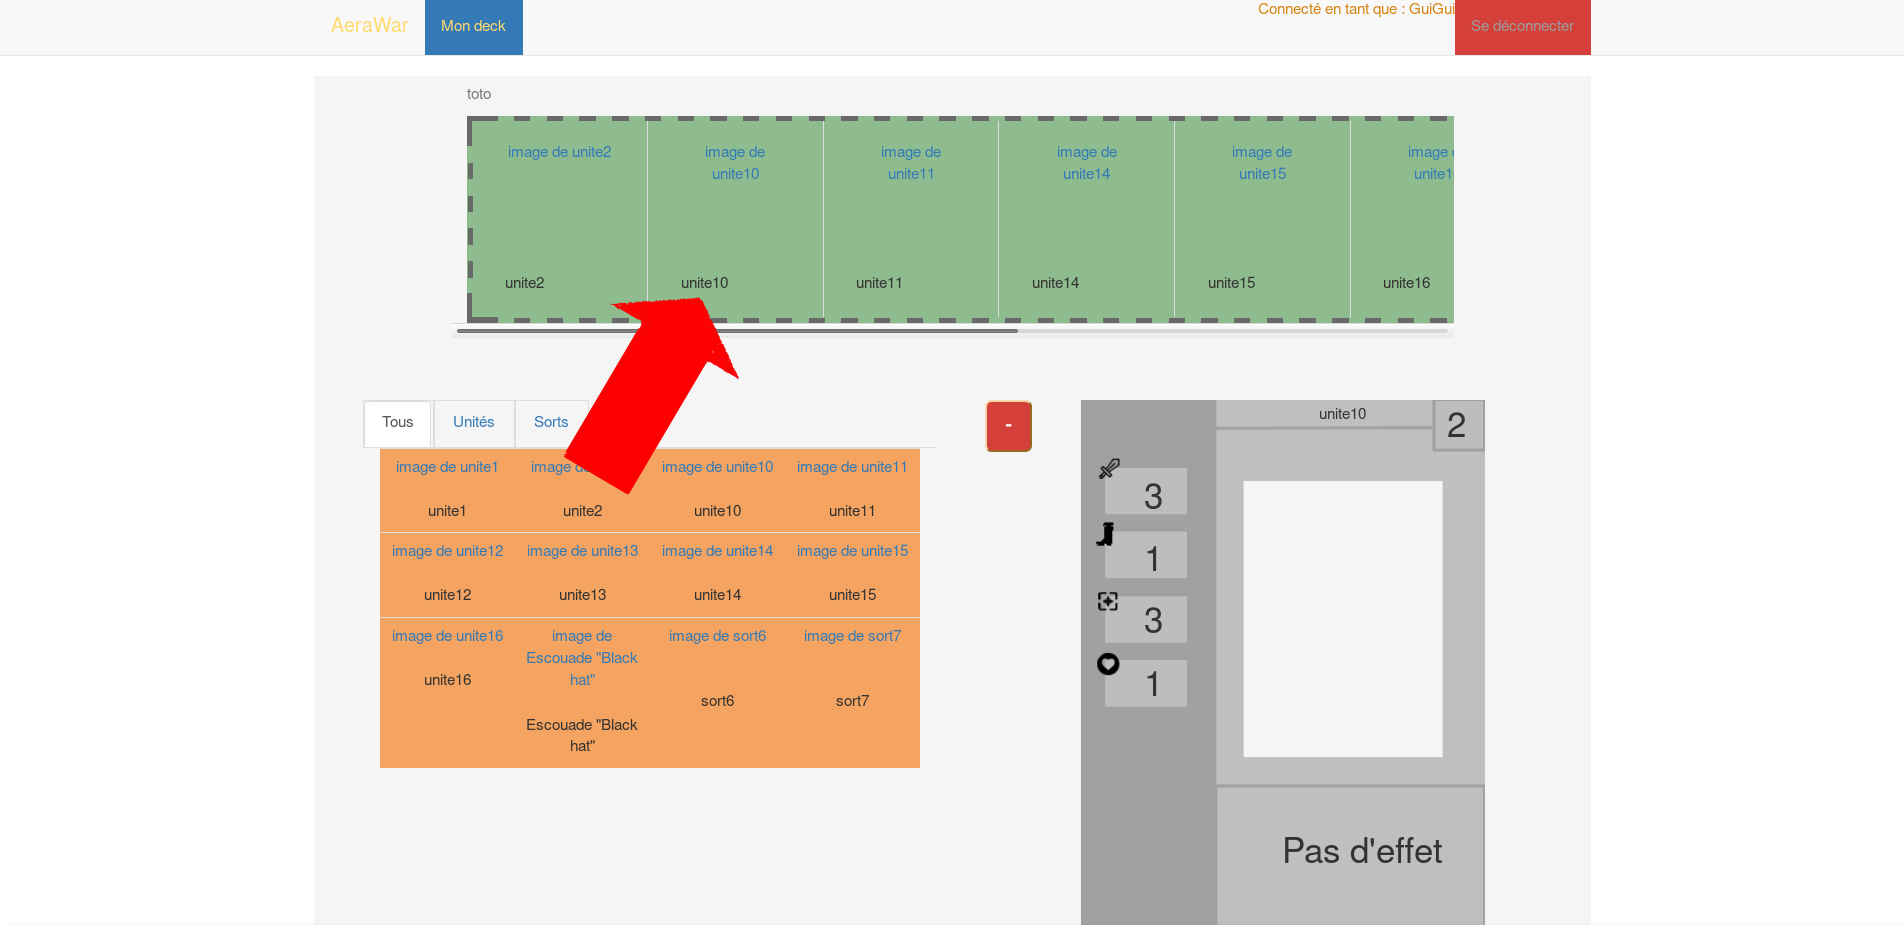
\includegraphics[scale=0.4]{Assets/add_deck.png}
      		\caption{Ajout d'une carte \textit{data wars}}
      		\label{fig2}
     		\end{center}
	\end{figure}

        
\end{document}  

